\documentclass[a4paper, oneside]{memoir}
\usepackage[utf8]{inputenc}
\usepackage[T1]{fontenc}
\usepackage{pifont}
\usepackage{amssymb}
\usepackage{fourier}
\usepackage[dvipsnames]{xcolor}
\usepackage{tikz}
\usepackage{pdfpages}
\usepackage[sfdefault]{roboto}
\usepackage{color}

% Styles
\tikzstyle{teamshare} = [below, text width=5.4cm, inner sep = 0.5cm, text=white, align=center]
\tikzstyle{cardtext} = [below, text width=5.9cm, inner sep = 0.25cm, text centered]
\setlrmarginsandblock{0.9cm}{*}{1}
\setulmarginsandblock{1.49cm}{*}{1}
\checkandfixthelayout[nearest]
\pagestyle{empty}

% Define Commands
\newcommand{\condition}[1]{\textbf{#1}}
\newcommand{\character}[1]{\textbf{#1}}
\newdimen\titlespacing
\titlespacing=0.15cm

% Define Seperators
\newcommand{\seperator}[1]{\\ \vspace{\titlespacing} \hrulefill {} \tiny \bfseries #1 \normalfont \normalsize \hrulefill \\ \vspace{\titlespacing}}
\newcommand{\seperatoraction}{\seperator{POWER}}
\newcommand{\seperatordescription}{\seperator{DESCRIPTION}}
\newcommand{\seperatorcondition}{\seperator{CONDITION}}
\newcommand{\seperatorwin}{\seperator{HOW TO WIN}}
\newcommand{\redwinsection}{
	\seperatorwin
	You win if \character{Harry Potter} does not gain the \condition{dead} condition due to \character{Voldemort}.
}
\newcommand{\greenwinsection}{
	\seperatorwin
	\small You win if \character{Harry Potter} gains the \condition{dead} condition due to the \character{Voldemort}.
}
\newcommand{\titlefrom}[1]{\\ \tiny > from #1 <\normalsize}

% Begin Document
\begin{document}
	
% New Page
\noindent 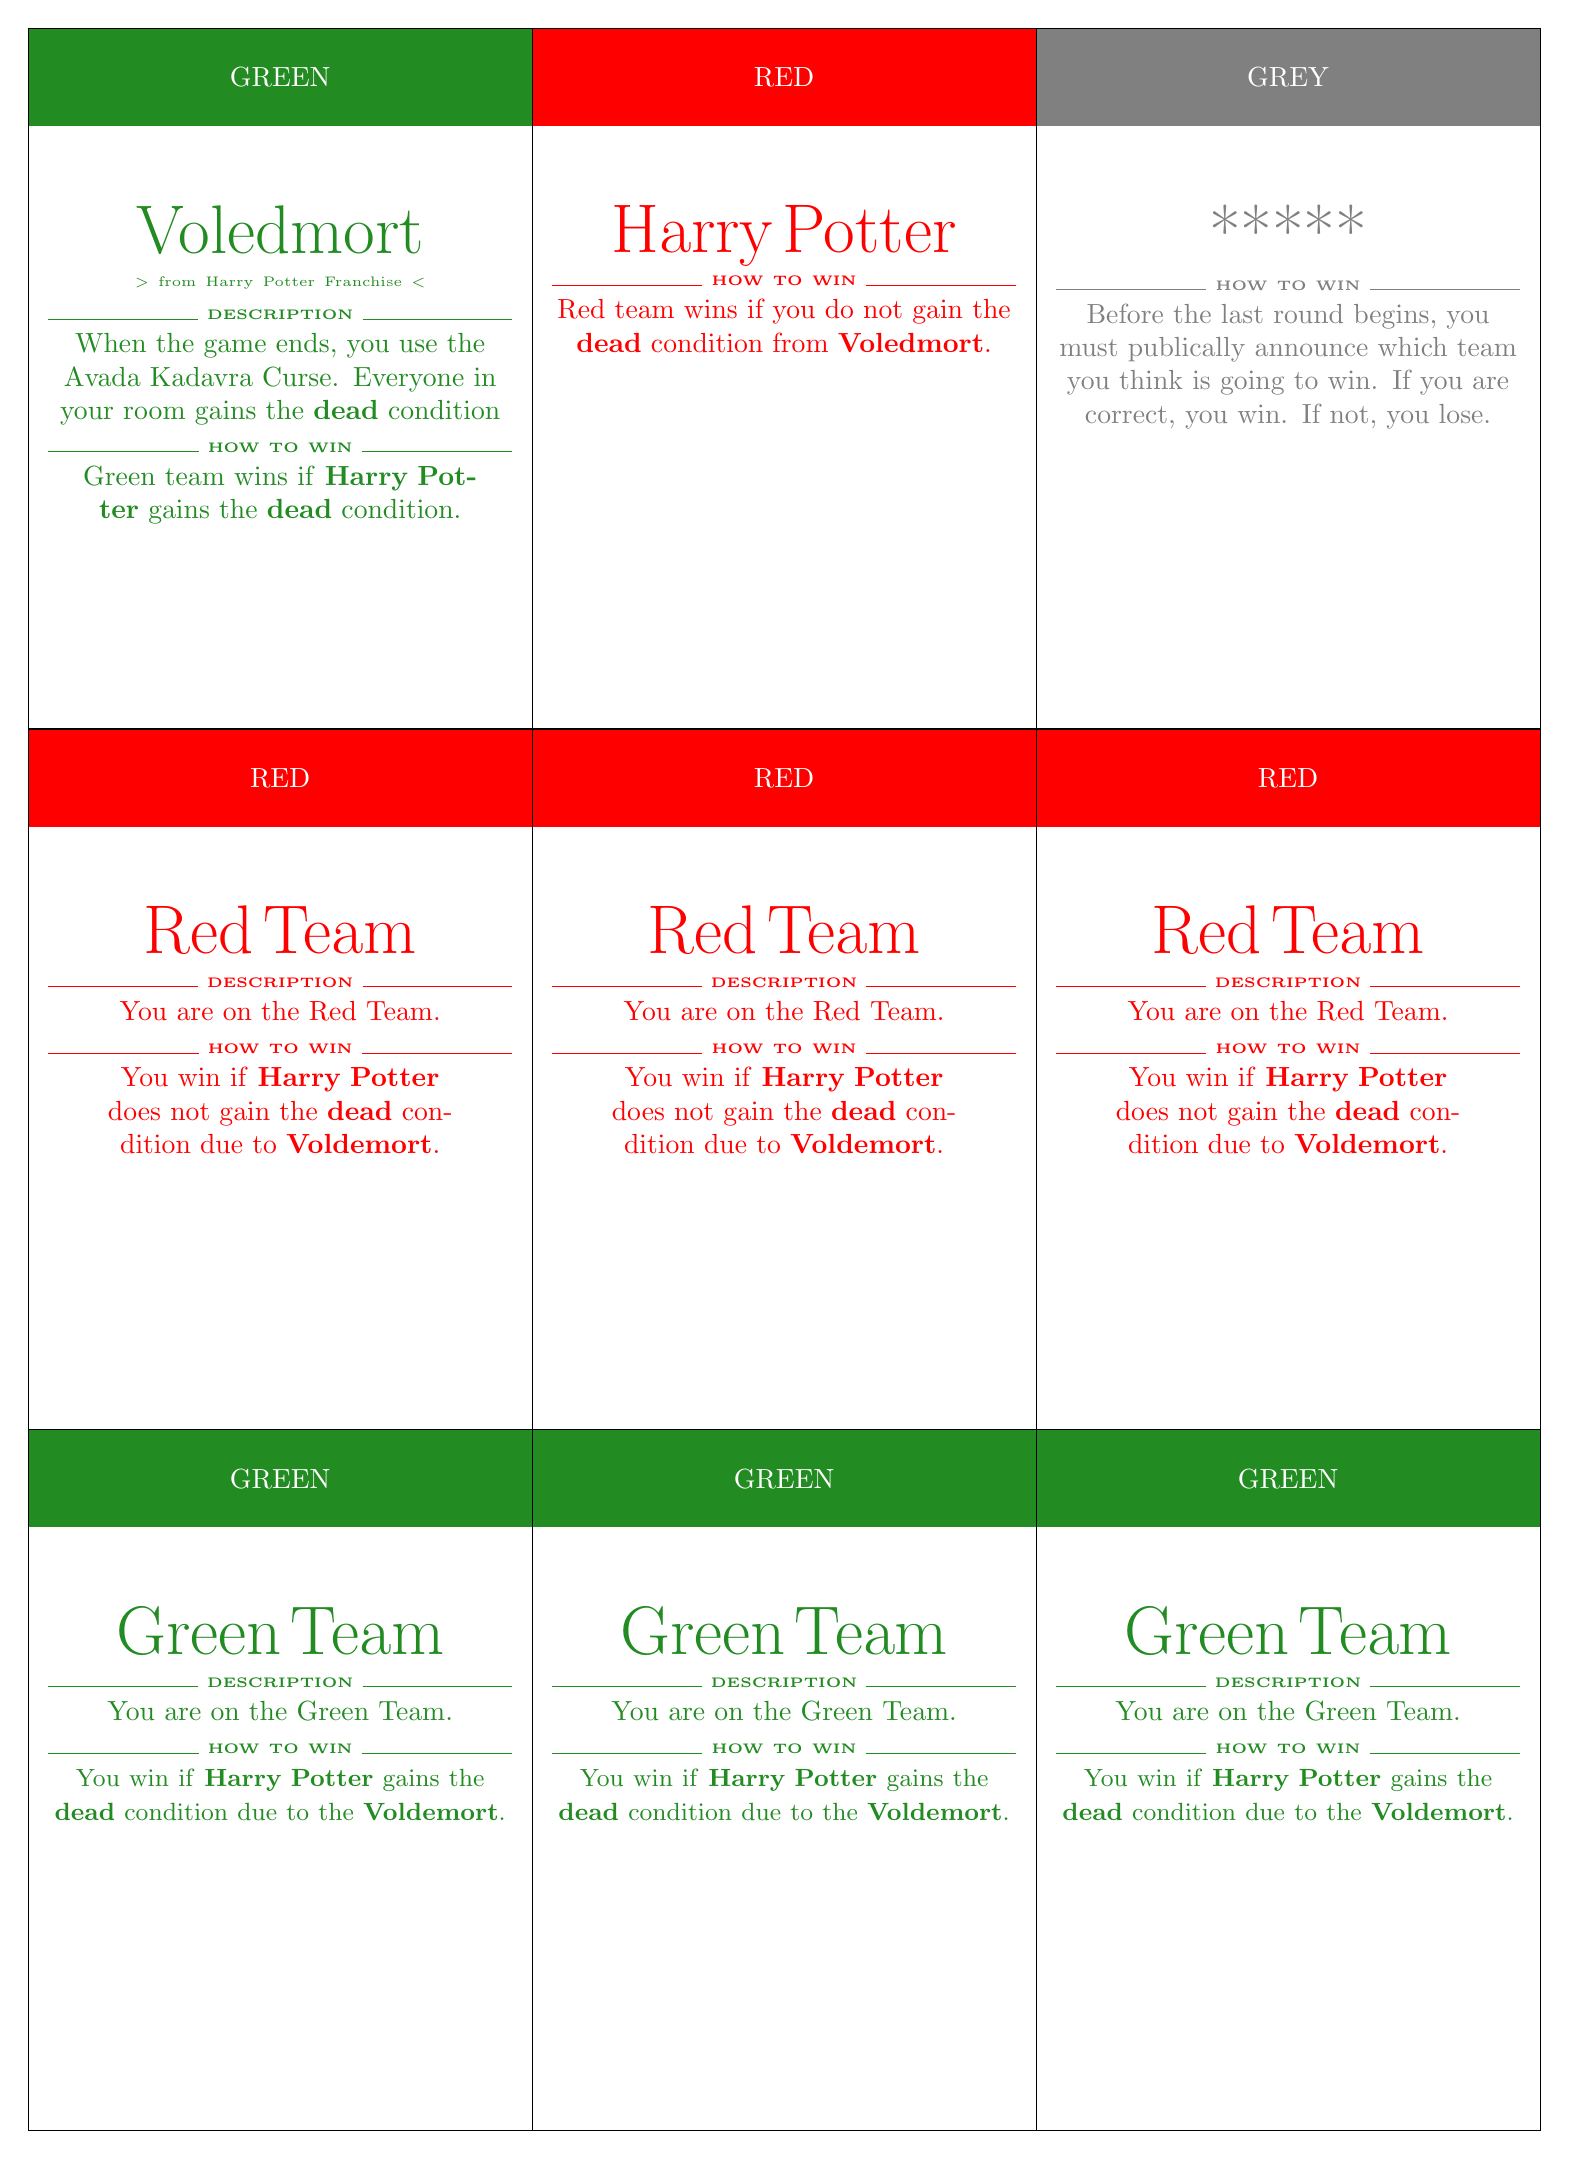
\begin{tikzpicture}[outer sep=0]

	% VOLDEMORT
	\node[teamshare, fill=ForestGreen] (1) at (3.2,26.7) {\HUGE GREEN};
	\node[cardtext, text=ForestGreen] at (3.2,24.7) {
		{\Huge Voledmort}
		\titlefrom{Harry Potter Franchise}
		\seperatordescription
		When the game ends, you use the Avada Kadavra Curse. Everyone in your room gains the \condition{dead} condition
		\seperatorwin
		Green team wins if \character{Harry Potter} gains the \condition{dead} condition.
	};
	
	% HARRY POTTER
	\node[teamshare, fill=red] at (9.6,26.7) {\HUGE RED};
	\node[cardtext, text=red] at (9.6,24.7) {
		{\Huge Harry Potter}
		\seperatorwin
		Red team wins if you do not gain the \condition{dead} condition from \character{Voledmort}.
	};
	
	% ******
	\node[teamshare, fill=gray] at (16,26.7) {\HUGE GREY};
	\node[cardtext, text=gray] at (16,24.7) {
		{\Huge *****}
		\seperatorwin
		Before the last round begins, you must publically announce which team you think is going to win. If you are correct, you win. If not, you lose.
	};
	
	% RED TEAM
	\node[teamshare, fill=red] at (3.2,17.8) {\HUGE RED};
	\node[cardtext, text=red] at (3.2,15.8) {
		{\Huge Red Team}
		\seperatordescription
		You are on the Red Team.
		\redwinsection
	};
	
	% RED TEAM
	\node[teamshare, fill=red] at (9.6,17.8) {\HUGE RED};
	\node[cardtext, text=red] at (9.6,15.8) {
		{\Huge Red Team}
		\seperatordescription
		You are on the Red Team.
		\redwinsection
	};
	
	% RED TEAM
	\node[teamshare, fill=red] at (16,17.8) {\HUGE RED};
	\node[cardtext, text=red] at (16,15.8) {
		{\Huge Red Team}
		\seperatordescription
		You are on the Red Team.
		\redwinsection
	};
	
	% GREEN TEAM
	\node[teamshare, fill=ForestGreen] at (3.2,8.9) {\HUGE GREEN};
	\node[cardtext, text=ForestGreen] at (3.2,6.9) {
		{\Huge Green Team}
		\seperatordescription
		You are on the Green Team.
		\greenwinsection
	};
	
	% GREEN TEAM
	\node[teamshare, fill=ForestGreen] at (9.6,8.9) {\HUGE GREEN};
	\node[cardtext, text=ForestGreen] at (9.6,6.9) {
		{\Huge Green Team}
		\seperatordescription
		You are on the Green Team.
		\greenwinsection
	};
	
	% GREEN TEAM
	\node[teamshare, fill=ForestGreen] at (16,8.9) {\HUGE GREEN};
	\node[cardtext, text=ForestGreen] at (16,6.9) {
		{\Huge Green Team}
		\seperatordescription
		You are on the Green Team.
		\greenwinsection
	};
	
	\draw (0,0) -- (19.2,0);
	\draw (0,8.9) -- (19.2,8.9);
	\draw (0,17.8) -- (19.2,17.8);
	\draw (0,26.7) -- (19.2,26.7);
	
	\draw (0,0) -- (0,26.7);
	\draw (6.4,0) -- (6.4,26.7);
	\draw (12.8,0) -- (12.8,26.7);
	\draw (19.2,0) -- (19.2,26.7);



\end{tikzpicture}

%Background is not my own. But courtesy of a user on BGG
\includepdf[pages={1}, angle=90]{cardsbackground.pdf}
\pagebreak

\noindent 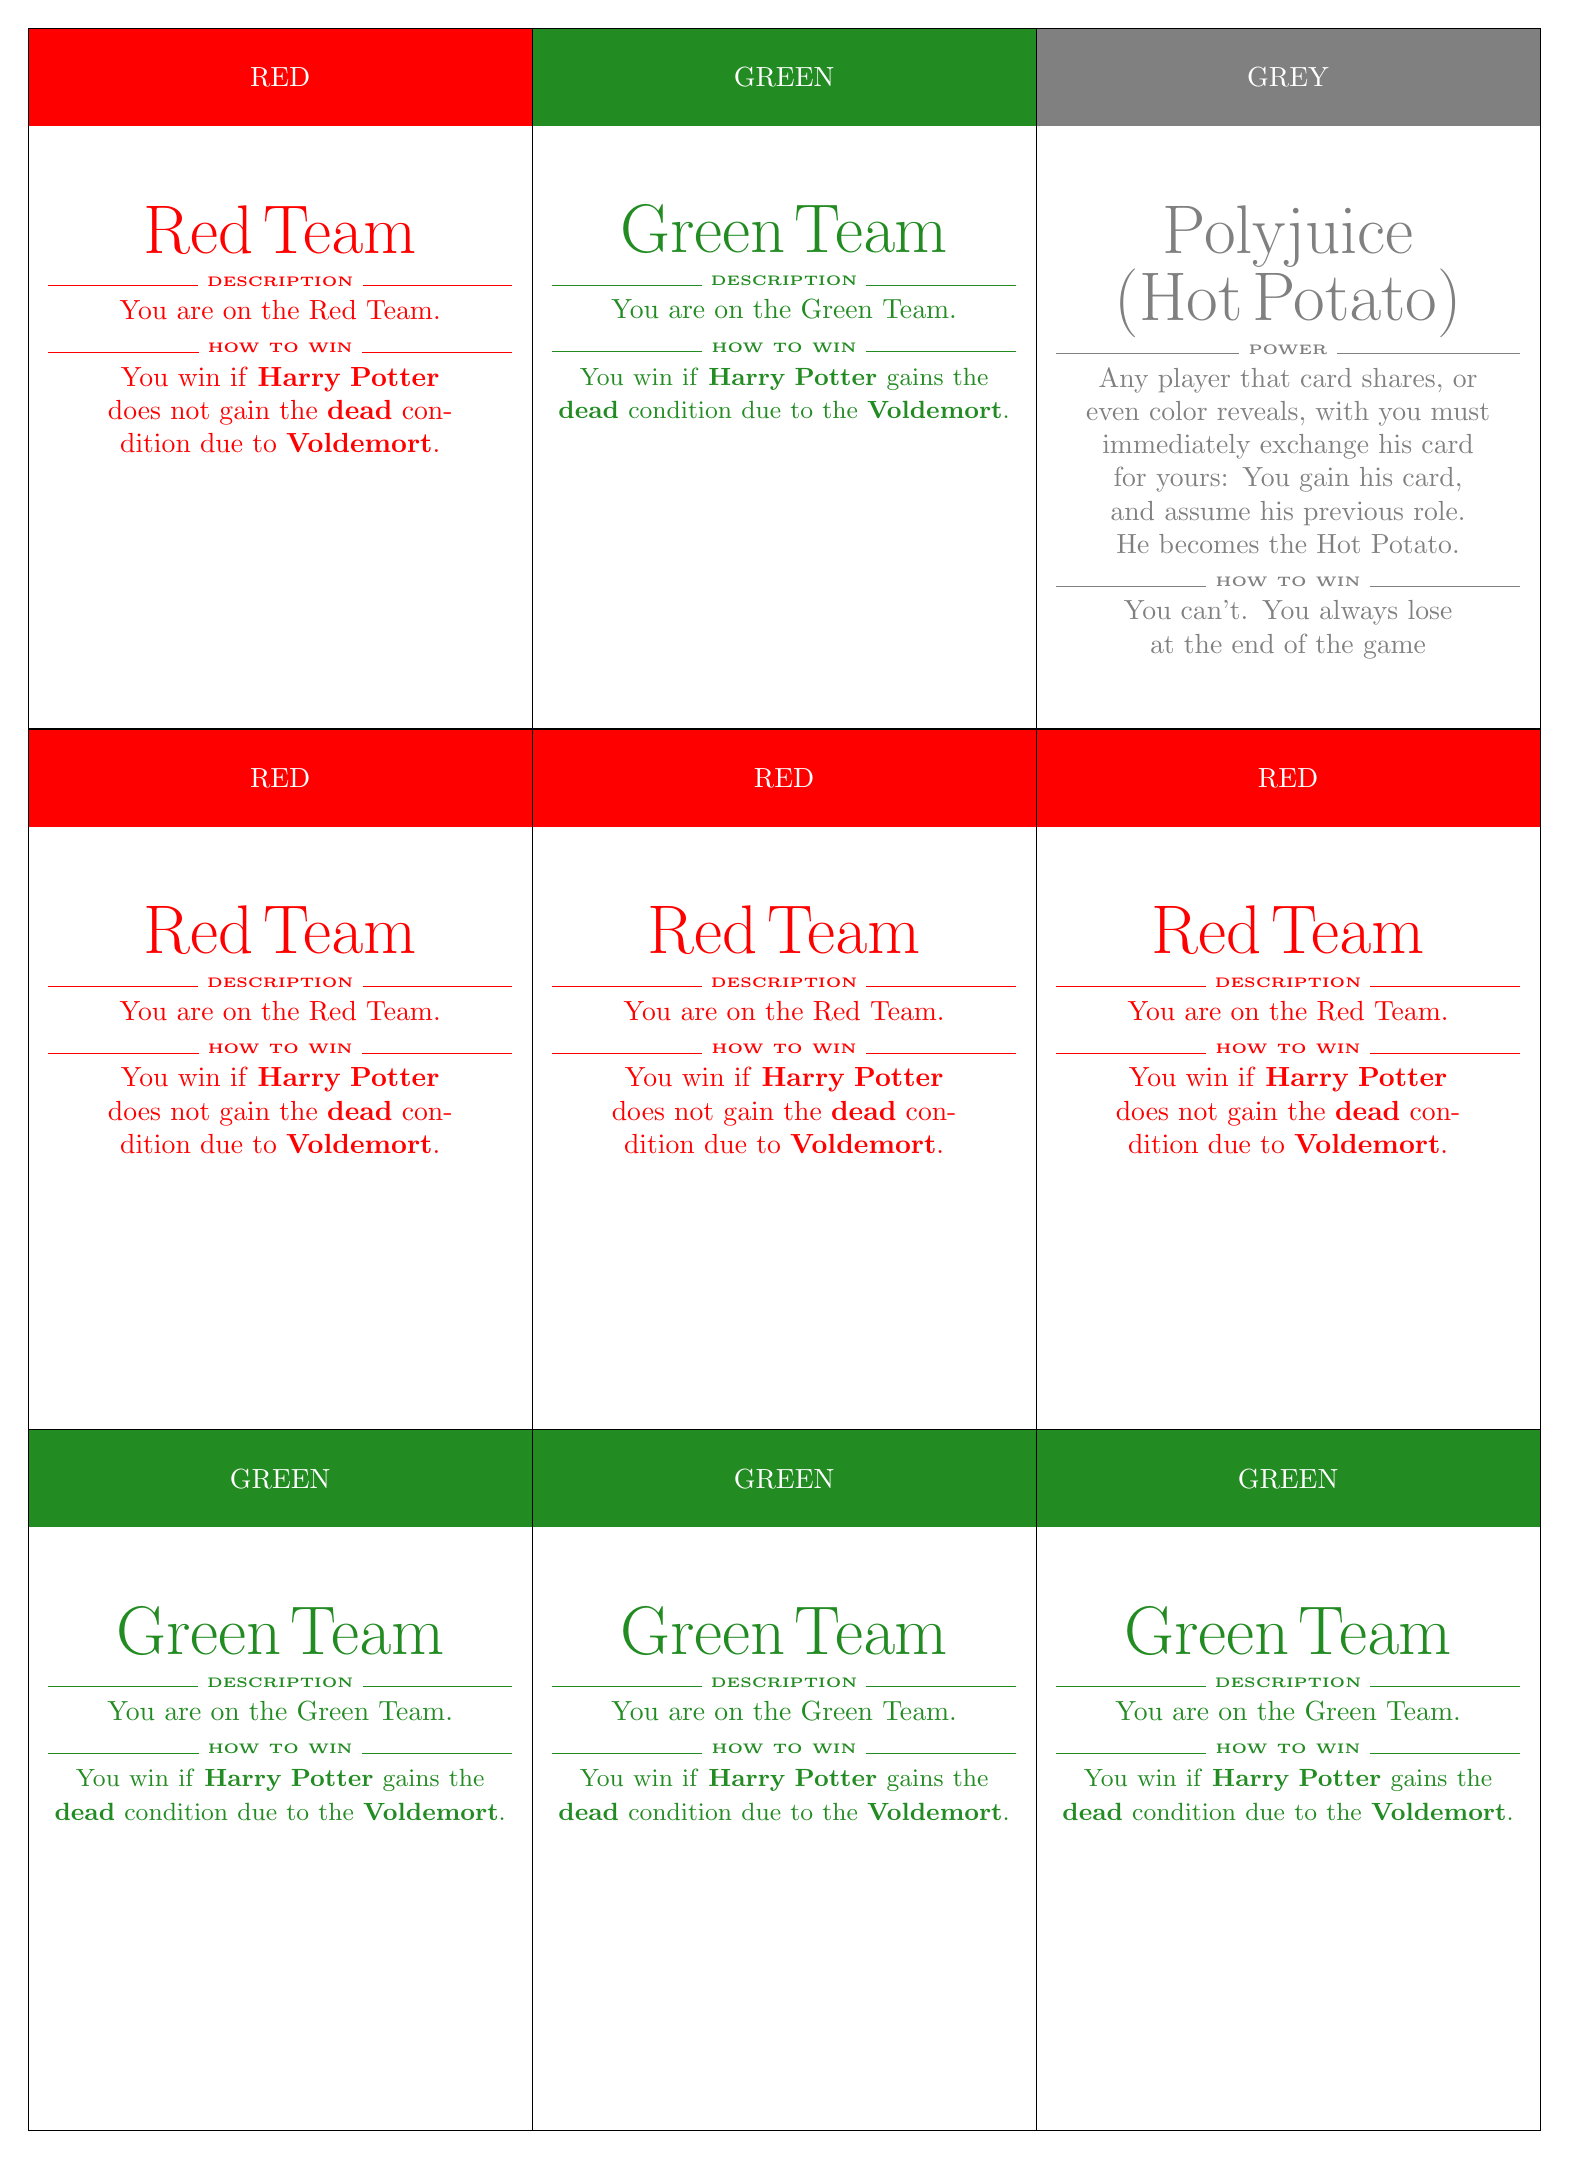
\begin{tikzpicture}[outer sep=0]

	% RED TEAM
	\node[teamshare, fill=red] (1) at (3.2,26.7) {\HUGE RED};
	\node[cardtext, text=red] at (3.2,24.7) {
		{\Huge Red Team}
		\seperatordescription
		You are on the Red Team.
		\redwinsection
	};
	
	% GREEN TEAM
	\node[teamshare, fill=ForestGreen] at (9.6,26.7) {\HUGE GREEN};
	\node[cardtext, text=ForestGreen] at (9.6,24.7) {
		{\Huge Green Team}
		\seperatordescription
		You are on the Green Team.
		\greenwinsection
	};
	
	% POLYJUICE POTATO
	\node[teamshare, fill=gray] at (16,26.7) {\HUGE GREY};
	\node[cardtext, text=gray] at (16,24.7) {
		{\Huge Polyjuice (Hot Potato)}
		\seperatoraction
		Any player that card shares, or even color reveals, with you must immediately exchange his card for yours: You gain his card, and assume his previous role. He becomes the Hot Potato.
		\seperatorwin
		You can't. You always lose at the end of the game	
	};
	
	% RED TEAM
	\node[teamshare, fill=red] at (3.2,17.8) {\HUGE RED};
	\node[cardtext, text=red] at (3.2,15.8) {
		{\Huge Red Team}
		\seperatordescription
		You are on the Red Team.
		\redwinsection
	};
	
	% RED TEAM
	\node[teamshare, fill=red] at (9.6,17.8) {\HUGE RED};
	\node[cardtext, text=red] at (9.6,15.8) {
		{\Huge Red Team}
		\seperatordescription
		You are on the Red Team.
		\redwinsection
	};
	
	% RED TEAM
	\node[teamshare, fill=red] at (16,17.8) {\HUGE RED};
	\node[cardtext, text=red] at (16,15.8) {
		{\Huge Red Team}
		\seperatordescription
		You are on the Red Team.
		\redwinsection
	};
	
	% GREEN TEAM
	\node[teamshare, fill=ForestGreen] at (3.2,8.9) {\HUGE GREEN};
	\node[cardtext, text=ForestGreen] at (3.2,6.9) {
		{\Huge Green Team}
		\seperatordescription
		You are on the Green Team.
		\greenwinsection
	};
	
	% GREEN TEAM
	\node[teamshare, fill=ForestGreen] at (9.6,8.9) {\HUGE GREEN};
	\node[cardtext, text=ForestGreen] at (9.6,6.9) {
		{\Huge Green Team}
		\seperatordescription
		You are on the Green Team.
		\greenwinsection
	};
	
	% GREEN TEAM
	\node[teamshare, fill=ForestGreen] at (16,8.9) {\HUGE GREEN};
	\node[cardtext, text=ForestGreen] at (16,6.9) {
		{\Huge Green Team}
		\seperatordescription
		You are on the Green Team.
		\greenwinsection
	};
	
	\draw (0,0) -- (19.2,0);
	\draw (0,8.9) -- (19.2,8.9);
	\draw (0,17.8) -- (19.2,17.8);
	\draw (0,26.7) -- (19.2,26.7);
	\draw (0,0) -- (0,26.7);
	\draw (6.4,0) -- (6.4,26.7);
	\draw (12.8,0) -- (12.8,26.7);
	\draw (19.2,0) -- (19.2,26.7);

\end{tikzpicture}

\includepdf[pages={1}, angle=90]{cardsbackground.pdf}
\pagebreak

\noindent 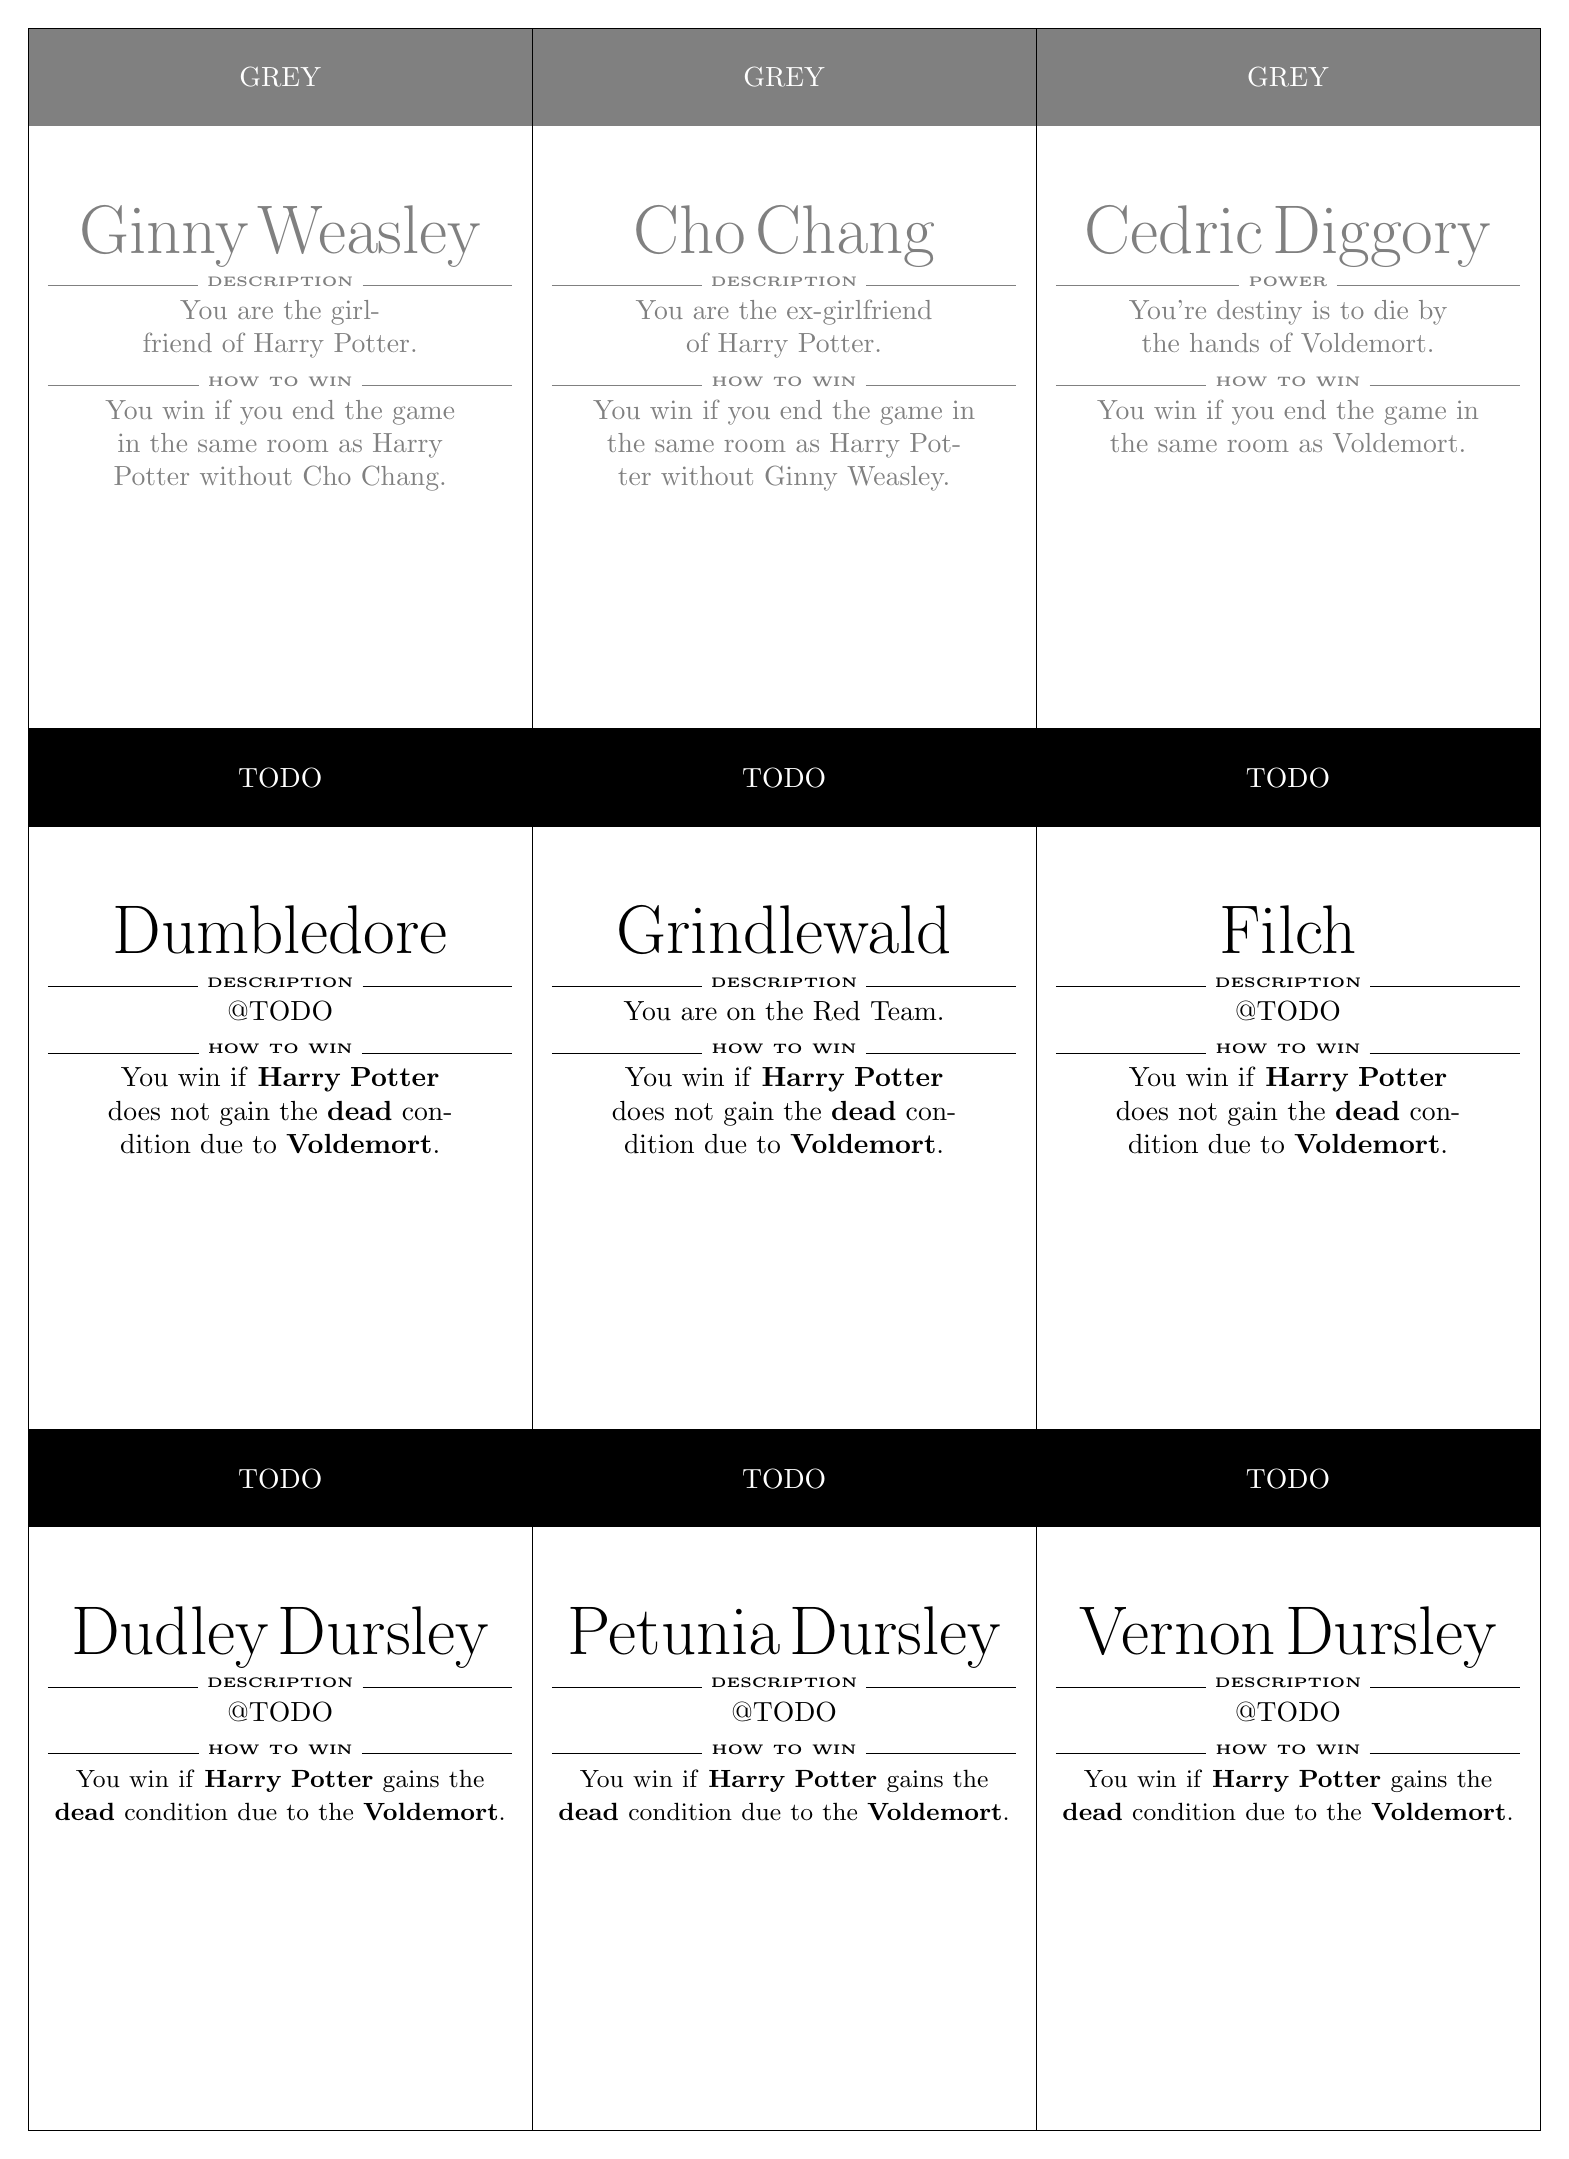
\begin{tikzpicture}[outer sep=0]

	% GINNY WEASLEY
	\node[teamshare, fill=gray] (1) at (3.2,26.7) {\HUGE GREY};
	\node[cardtext, text=gray] at (3.2,24.7) {
		{\Huge Ginny Weasley}
		\seperatordescription
		You are the girlfriend of Harry Potter.
		\seperatorwin
		You win if you end the game in the same room as Harry Potter without Cho Chang.
	};
	
	% CHO CHANG
	\node[teamshare, fill=gray] at (9.6,26.7) {\HUGE GREY};
	\node[cardtext, text=gray] at (9.6,24.7) {
		{\Huge Cho Chang}
		\seperatordescription
		You are the ex-girlfriend of Harry Potter.
		\seperatorwin
		You win if you end the game in the same room as Harry Potter without Ginny Weasley.
	};
	
	% CEDRIC DIGGORY
	\node[teamshare, fill=gray] at (16,26.7) {\HUGE GREY};
	\node[cardtext, text=gray] at (16,24.7) {
		{\Huge Cedric Diggory}
		\seperatoraction
		You're destiny is to die by the hands of Voldemort.
		\seperatorwin
		You win if you end the game in the same room as Voldemort.
	};
	
	% DUMBLEDORE
	\node[teamshare, fill=black] at (3.2,17.8) {\HUGE TODO};
	\node[cardtext, text=black] at (3.2,15.8) {
		{\Huge Dumbledore}
		\seperatordescription
		@TODO
		\redwinsection
	};
	
	% GRINDLEWALD
	\node[teamshare, fill=black] at (9.6,17.8) {\HUGE TODO};
	\node[cardtext, text=black] at (9.6,15.8) {
		{\Huge Grindlewald}
		\seperatordescription
		You are on the Red Team.
		\redwinsection
	};
	
	% FILCH
	\node[teamshare, fill=black] at (16,17.8) {\HUGE TODO};
	\node[cardtext, text=black] at (16,15.8) {
		{\Huge Filch}
		\seperatordescription
		@TODO
		\redwinsection
	};
	
	% DUDLY DURSLEY
	\node[teamshare, fill=black] at (3.2,8.9) {\HUGE TODO};
	\node[cardtext, text=black] at (3.2,6.9) {
		{\Huge Dudley Dursley}
		\seperatordescription
		@TODO
		\greenwinsection
	};
	
	% PETUNIA DURSLEY
	\node[teamshare, fill=black] at (9.6,8.9) {\HUGE TODO};
	\node[cardtext, text=black] at (9.6,6.9) {
		{\Huge Petunia Dursley}
		\seperatordescription
		@TODO
		\greenwinsection
	};
	
	% VERNON DURSLEY
	\node[teamshare, fill=black] at (16,8.9) {\HUGE TODO};
	\node[cardtext, text=black] at (16,6.9) {
		{\Huge Vernon Dursley}
		\seperatordescription
		@TODO
		\greenwinsection
	};
	
	\draw (0,0) -- (19.2,0);
	\draw (0,8.9) -- (19.2,8.9);
	\draw (0,17.8) -- (19.2,17.8);
	\draw (0,26.7) -- (19.2,26.7);
	\draw (0,0) -- (0,26.7);
	\draw (6.4,0) -- (6.4,26.7);
	\draw (12.8,0) -- (12.8,26.7);
	\draw (19.2,0) -- (19.2,26.7);

\end{tikzpicture}
\includepdf[pages={1}, angle=90]{cardsbackground.pdf}
\pagebreak

\noindent 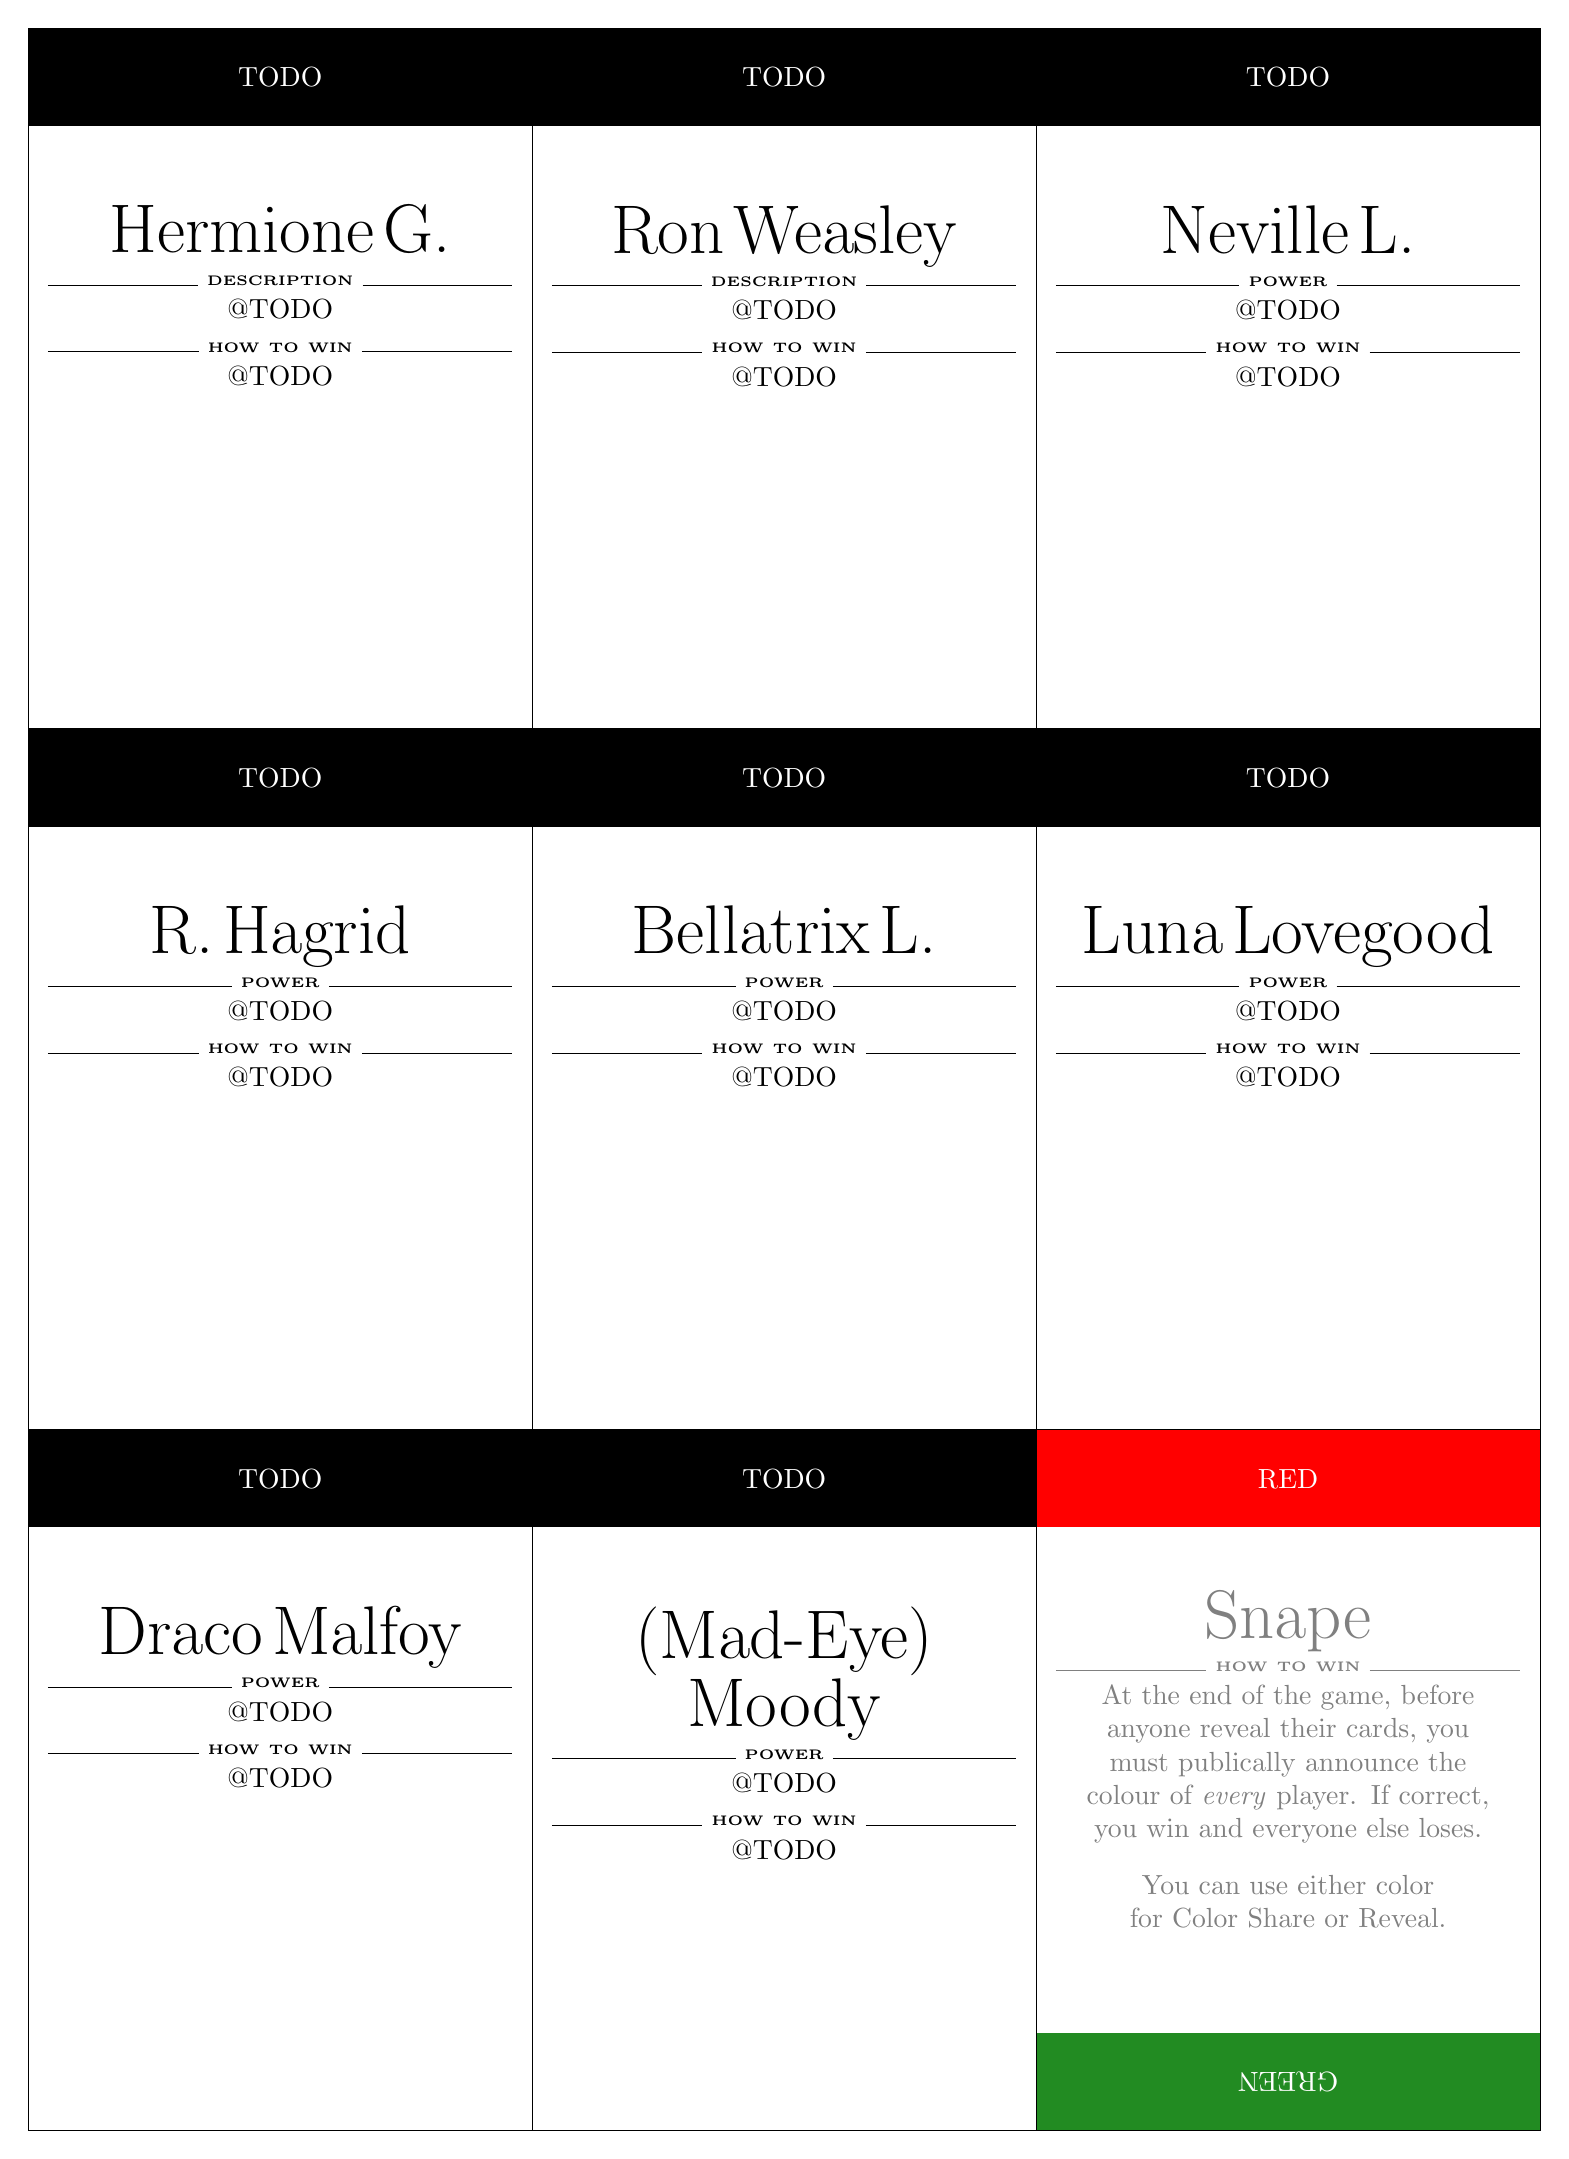
\begin{tikzpicture}[outer sep=0]
	
	% HERMIONE G.
	\node[teamshare, fill=black] (1) at (3.2,26.7) {\HUGE TODO};
	\node[cardtext, text=black] at (3.2,24.7) {
		{\Huge Hermione G.}
		\seperatordescription
		@TODO
		\seperatorwin
		@TODO
	};
	
	% RON WEASLEY
	\node[teamshare, fill=black] at (9.6,26.7) {\HUGE TODO};
	\node[cardtext, text=black] at (9.6,24.7) {
		{\Huge Ron Weasley}
		\seperatordescription
		@TODO
		\seperatorwin
		@TODO
	};
	
	% NEVILLE LONGBOTTOM
	\node[teamshare, fill=black] at (16,26.7) {\HUGE TODO};
	\node[cardtext, text=black] at (16,24.7) {
		{\Huge Neville L.}
		\seperatoraction
		@TODO
		\seperatorwin
		@TODO
	};
	
	% RUBEAS HAGRID
	\node[teamshare, fill=black] at (3.2,17.8) {\HUGE TODO};
	\node[cardtext, text=black] at (3.2,15.8) {
		{\Huge R. Hagrid}
		\seperatoraction
		@TODO
		\seperatorwin
		@TODO
	};
	
	% BELLATRIX LESTRANGE
	\node[teamshare, fill=black] at (9.6,17.8) {\HUGE TODO};
	\node[cardtext, text=black] at (9.6,15.8) {
		{\Huge Bellatrix L.}
		\seperatoraction
		@TODO
		\seperatorwin
		@TODO
	};
	
	% LUNA LOVEGOOD
	\node[teamshare, fill=black] at (16,17.8) {\HUGE TODO};
	\node[cardtext, text=black] at (16,15.8) {
		{\Huge Luna Lovegood}
		\seperatoraction
		@TODO
		\seperatorwin
		@TODO
	};
	
	% DRACO MALFOY
	\node[teamshare, fill=black] at (3.2,8.9) {\HUGE TODO};
	\node[cardtext, text=black] at (3.2,6.9) {
		{\Huge Draco Malfoy}
		\seperatoraction
		@TODO
		\seperatorwin
		@TODO
	};
	
	% MAD-EYE MOODY
	\node[teamshare, fill=black] at (9.6,8.9) {\HUGE TODO};
	\node[cardtext, text=black] at (9.6,6.9) {
		{\Huge (Mad-Eye) Moody}
		\seperatoraction
		@TODO
		\seperatorwin
		@TODO
	};
	
	% SNAPE
	\node[teamshare, fill=red] at (16,8.9) {\HUGE RED};
	\node[teamshare, fill=ForestGreen,rotate=180] at (16,0) {\HUGE GREEN};
	\node[cardtext, text=gray] at (16,7.1) {
		{\Huge Snape}
		\seperatorwin
		At the end of the game, before anyone reveal their cards, you must publically announce the colour of \emph{every} player. If correct, you win and everyone else loses.
		\\\vspace{0.3cm}
		You can use either color for Color Share or Reveal.
	};
	
	\draw (0,0) -- (19.2,0);
	\draw (0,8.9) -- (19.2,8.9);
	\draw (0,17.8) -- (19.2,17.8);
	\draw (0,26.7) -- (19.2,26.7);
	\draw (0,0) -- (0,26.7);
	\draw (6.4,0) -- (6.4,26.7);
	\draw (12.8,0) -- (12.8,26.7);
	\draw (19.2,0) -- (19.2,26.7);

\end{tikzpicture}
\includepdf[pages={1}, angle=90]{cardsbackground.pdf}
\pagebreak

\noindent 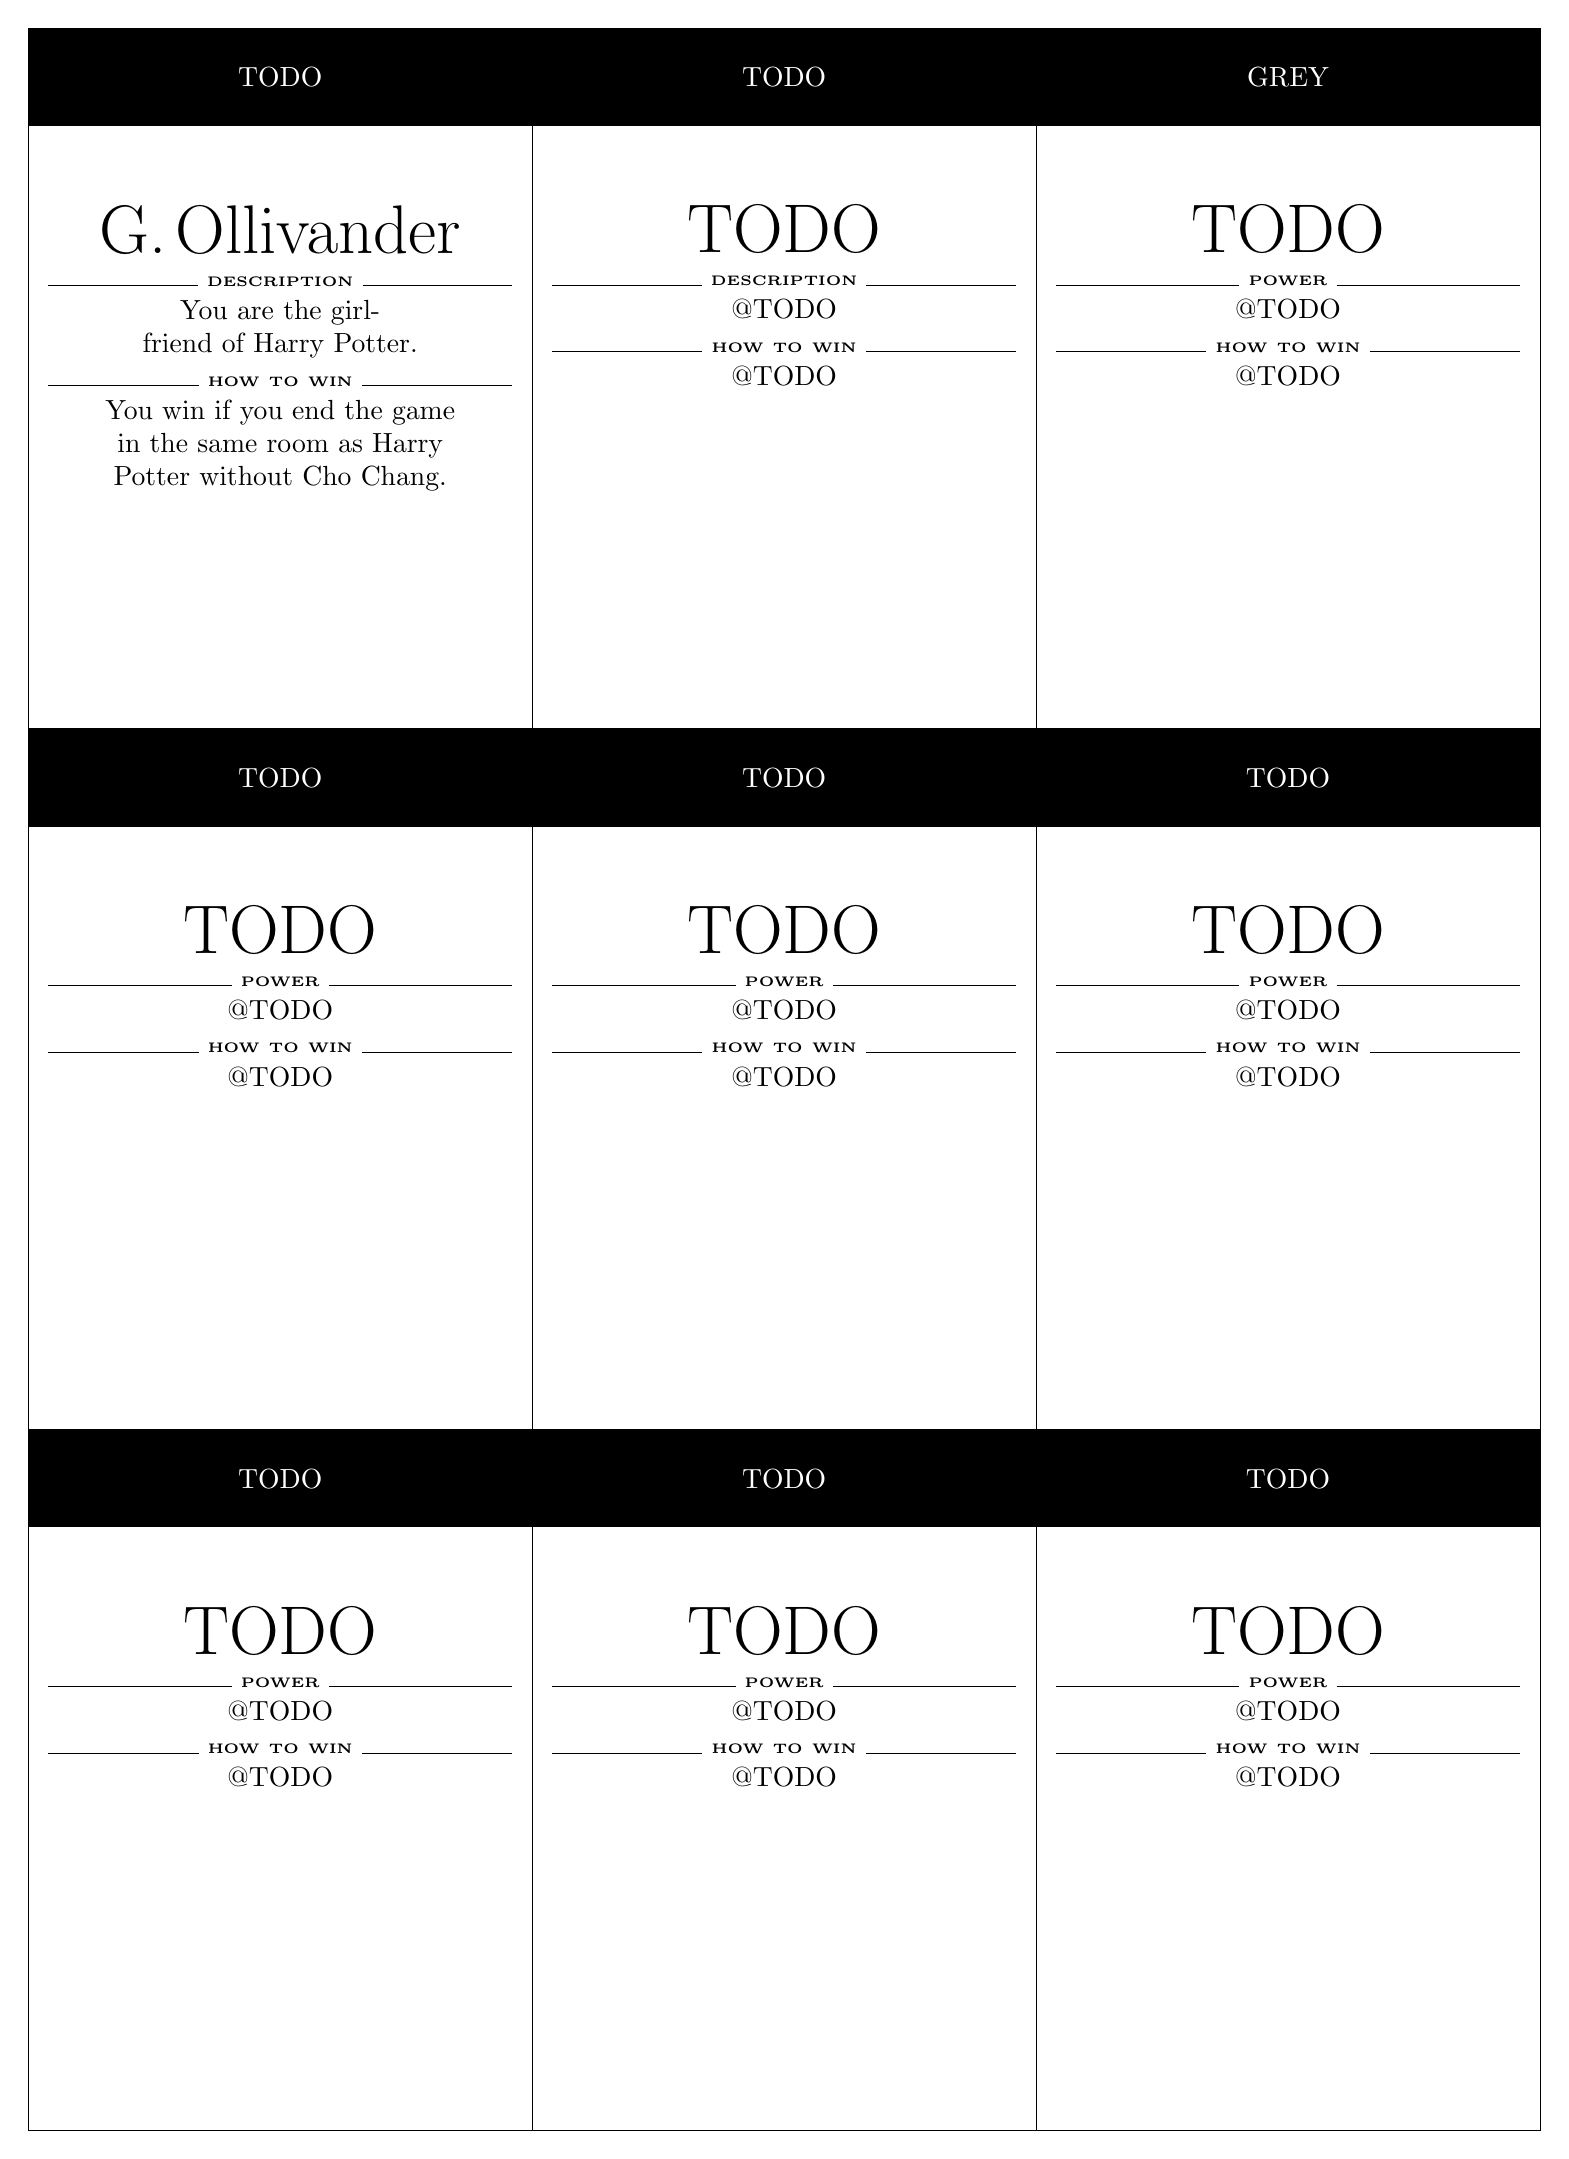
\begin{tikzpicture}[outer sep=0]

	% Garrick Ollivander
	\node[teamshare, fill=black] (1) at (3.2,26.7) {\HUGE TODO};
	\node[cardtext, text=black] at (3.2,24.7) {
		{\Huge G. Ollivander }
		\seperatordescription
		You are the girlfriend of Harry Potter.
		\seperatorwin
		You win if you end the game in the same room as Harry Potter without Cho Chang.
	};
	
	% TODO
	\node[teamshare, fill=black] at (9.6,26.7) {\HUGE TODO};
	\node[cardtext, text=black] at (9.6,24.7) {
		{\Huge TODO}
		\seperatordescription
		@TODO
		\seperatorwin
		@TODO
	};
	
	% TODO
	\node[teamshare, fill=black] at (16,26.7) {\HUGE GREY};
	\node[cardtext, text=black] at (16,24.7) {
		{\Huge TODO}
		\seperatoraction
		@TODO
		\seperatorwin
		@TODO
	};
	
	% TODO
	\node[teamshare, fill=black] at (3.2,17.8) {\HUGE TODO};
	\node[cardtext, text=black] at (3.2,15.8) {
		{\Huge TODO}
		\seperatoraction
		@TODO
		\seperatorwin
		@TODO
	};
	
	% TODO
	\node[teamshare, fill=black] at (9.6,17.8) {\HUGE TODO};
	\node[cardtext, text=black] at (9.6,15.8) {
		{\Huge TODO}
		\seperatoraction
		@TODO
		\seperatorwin
		@TODO
	};
	
	% TODO
	\node[teamshare, fill=black] at (16,17.8) {\HUGE TODO};
	\node[cardtext, text=black] at (16,15.8) {
		{\Huge TODO}
		\seperatoraction
		@TODO
		\seperatorwin
		@TODO
	};
	
	% TODO
	\node[teamshare, fill=black] at (3.2,8.9) {\HUGE TODO};
	\node[cardtext, text=black] at (3.2,6.9) {
		{\Huge TODO}
		\seperatoraction
		@TODO
		\seperatorwin
		@TODO
	};
	
	% TODO
	\node[teamshare, fill=black] at (9.6,8.9) {\HUGE TODO};
	\node[cardtext, text=black] at (9.6,6.9) {
		{\Huge TODO}
		\seperatoraction
		@TODO
		\seperatorwin
		@TODO
	};
	
	% TODO
	\node[teamshare, fill=black] at (16,8.9) {\HUGE TODO};
	\node[cardtext, text=black] at (16,6.9) {
		{\Huge TODO}
		\seperatoraction
		@TODO
		\seperatorwin
		@TODO
	};
	
	\draw (0,0) -- (19.2,0);
	\draw (0,8.9) -- (19.2,8.9);
	\draw (0,17.8) -- (19.2,17.8);
	\draw (0,26.7) -- (19.2,26.7);
	\draw (0,0) -- (0,26.7);
	\draw (6.4,0) -- (6.4,26.7);
	\draw (12.8,0) -- (12.8,26.7);
	\draw (19.2,0) -- (19.2,26.7);

\end{tikzpicture}
\includepdf[pages={1}, angle=90]{cardsbackground.pdf}
\pagebreak

\noindent 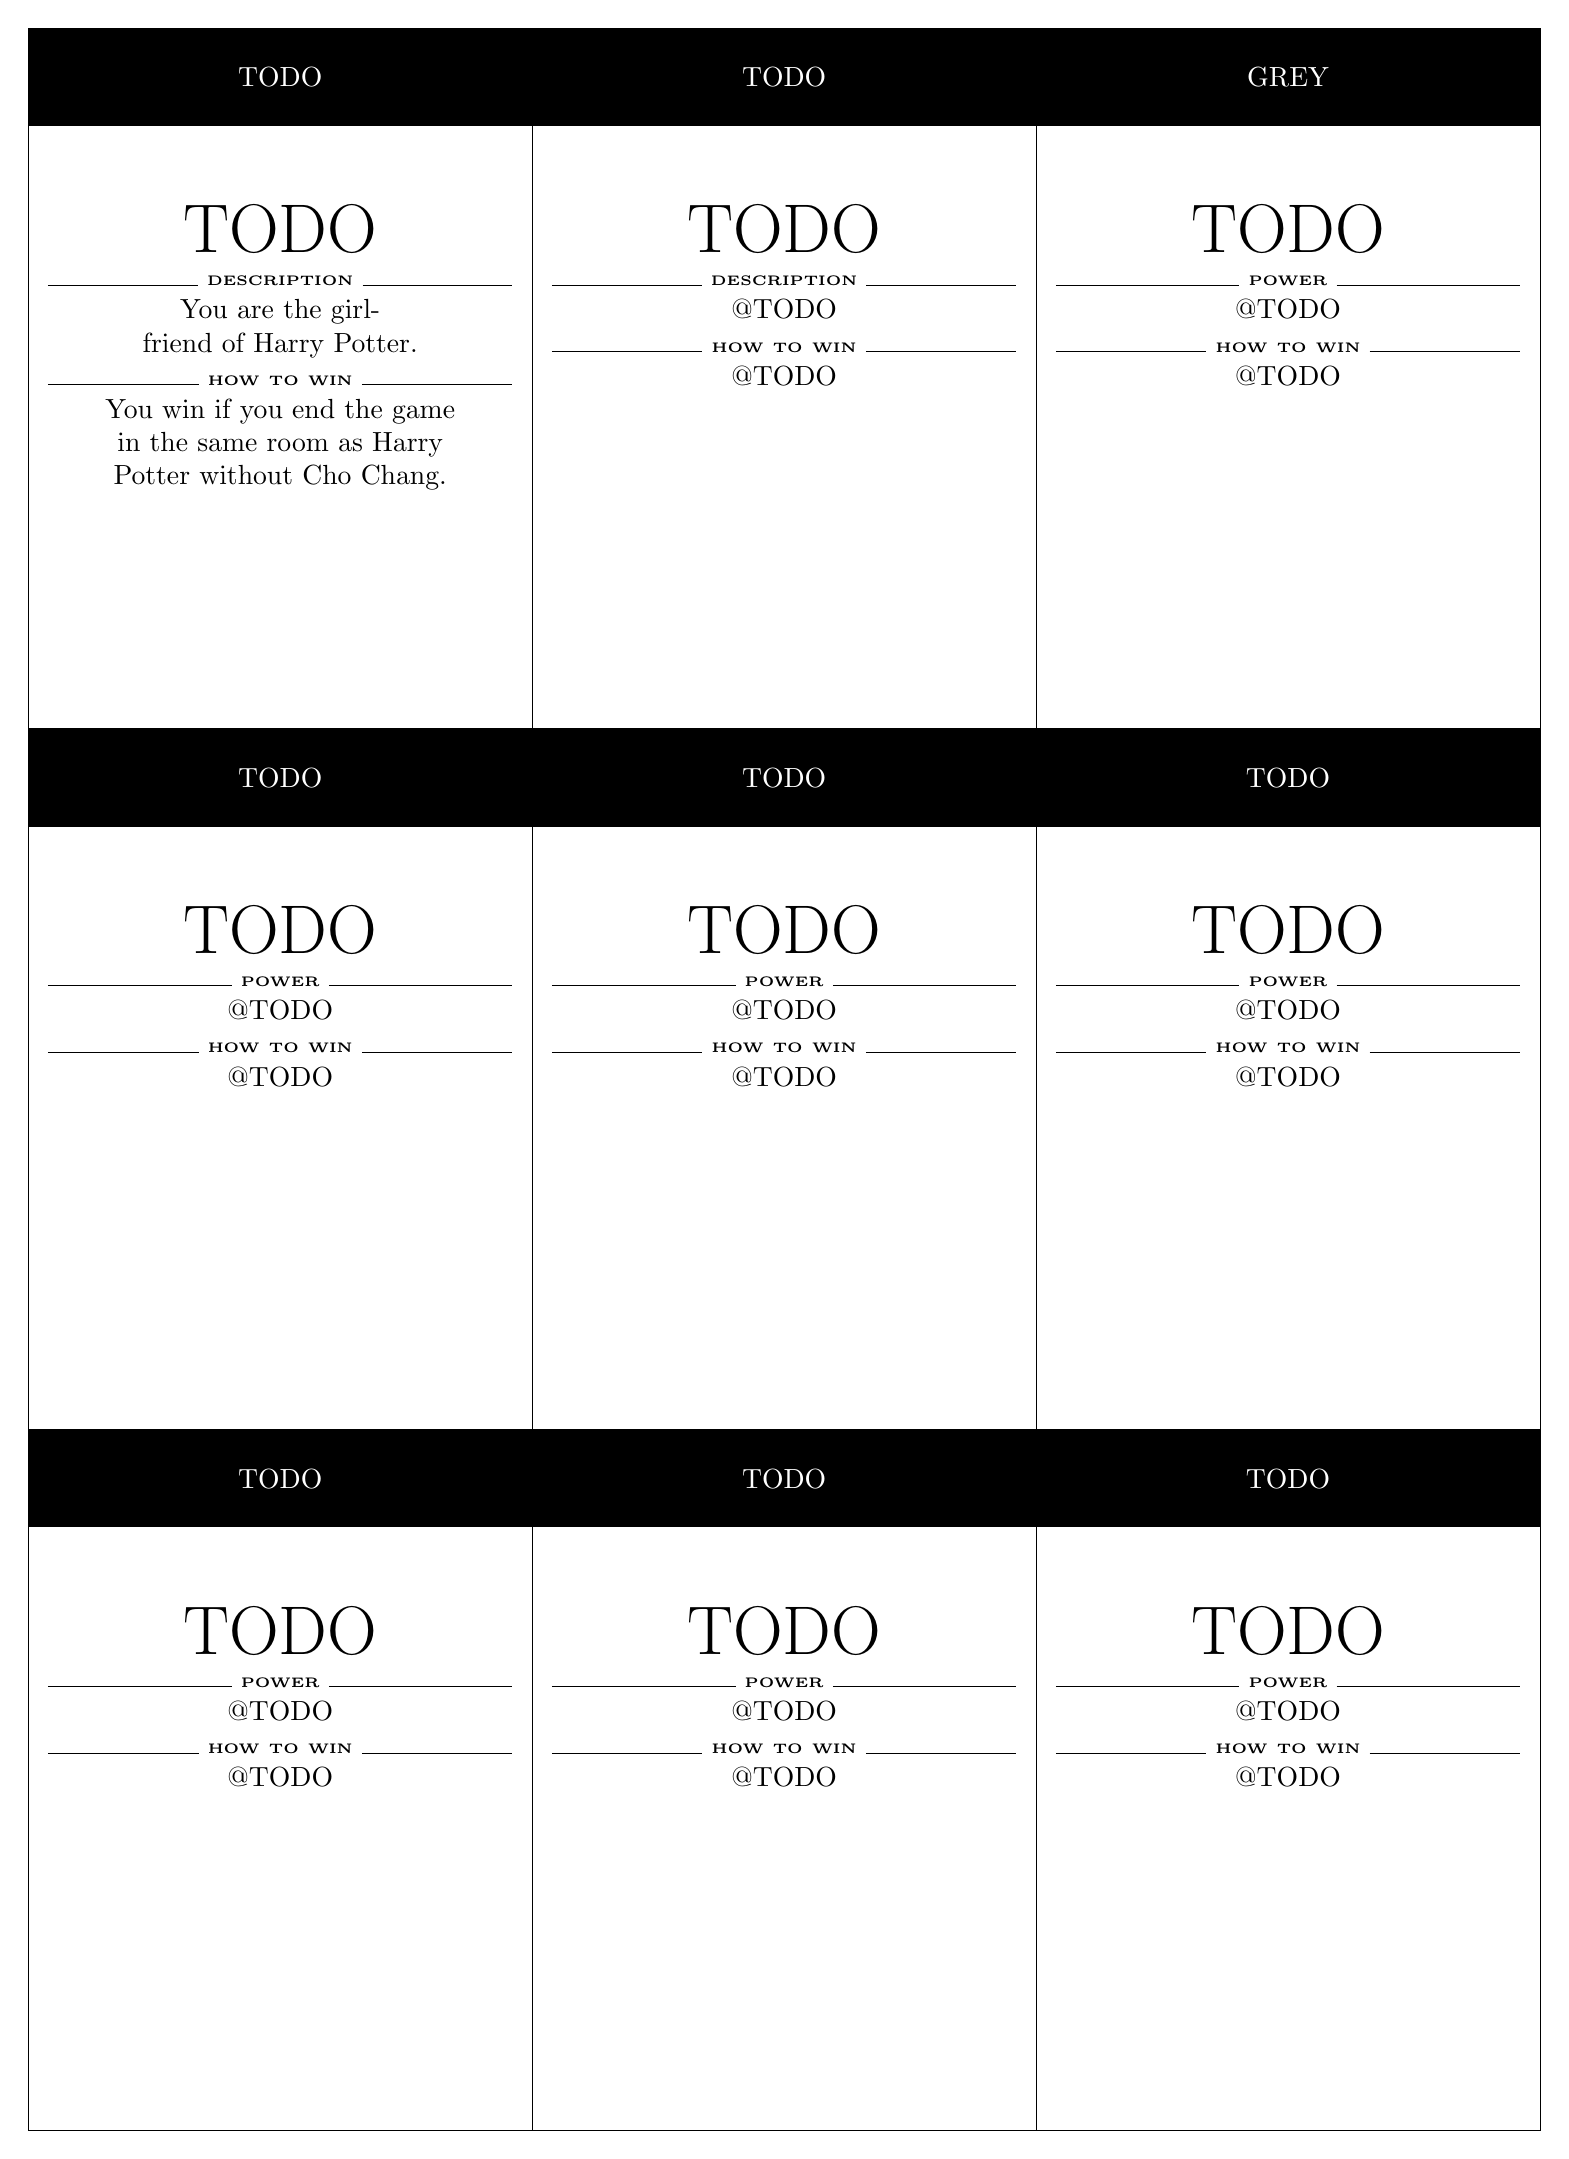
\begin{tikzpicture}[outer sep=0]

	% TODO
	\node[teamshare, fill=black] (1) at (3.2,26.7) {\HUGE TODO};
	\node[cardtext, text=black] at (3.2,24.7) {
		{\Huge TODO}
		\seperatordescription
		You are the girlfriend of Harry Potter.
		\seperatorwin
		You win if you end the game in the same room as Harry Potter without Cho Chang.
	};
	
	% TODO
	\node[teamshare, fill=black] at (9.6,26.7) {\HUGE TODO};
	\node[cardtext, text=black] at (9.6,24.7) {
		{\Huge TODO}
		\seperatordescription
		@TODO
		\seperatorwin
		@TODO
	};
	
	% TODO
	\node[teamshare, fill=black] at (16,26.7) {\HUGE GREY};
	\node[cardtext, text=black] at (16,24.7) {
		{\Huge TODO}
		\seperatoraction
		@TODO
		\seperatorwin
		@TODO
	};
	
	% TODO
	\node[teamshare, fill=black] at (3.2,17.8) {\HUGE TODO};
	\node[cardtext, text=black] at (3.2,15.8) {
		{\Huge TODO}
		\seperatoraction
		@TODO
		\seperatorwin
		@TODO
	};
	
	% TODO
	\node[teamshare, fill=black] at (9.6,17.8) {\HUGE TODO};
	\node[cardtext, text=black] at (9.6,15.8) {
		{\Huge TODO}
		\seperatoraction
		@TODO
		\seperatorwin
		@TODO
	};
	
	% TODO
	\node[teamshare, fill=black] at (16,17.8) {\HUGE TODO};
	\node[cardtext, text=black] at (16,15.8) {
		{\Huge TODO}
		\seperatoraction
		@TODO
		\seperatorwin
		@TODO
	};
	
	% TODO
	\node[teamshare, fill=black] at (3.2,8.9) {\HUGE TODO};
	\node[cardtext, text=black] at (3.2,6.9) {
		{\Huge TODO}
		\seperatoraction
		@TODO
		\seperatorwin
		@TODO
	};
	
	% TODO
	\node[teamshare, fill=black] at (9.6,8.9) {\HUGE TODO};
	\node[cardtext, text=black] at (9.6,6.9) {
		{\Huge TODO}
		\seperatoraction
		@TODO
		\seperatorwin
		@TODO
	};
	
	% TODO
	\node[teamshare, fill=black] at (16,8.9) {\HUGE TODO};
	\node[cardtext, text=black] at (16,6.9) {
		{\Huge TODO}
		\seperatoraction
		@TODO
		\seperatorwin
		@TODO
	};
	
	\draw (0,0) -- (19.2,0);
	\draw (0,8.9) -- (19.2,8.9);
	\draw (0,17.8) -- (19.2,17.8);
	\draw (0,26.7) -- (19.2,26.7);
	\draw (0,0) -- (0,26.7);
	\draw (6.4,0) -- (6.4,26.7);
	\draw (12.8,0) -- (12.8,26.7);
	\draw (19.2,0) -- (19.2,26.7);


\end{tikzpicture}
\includepdf[pages={1}, angle=90]{cardsbackground.pdf}








\end{document}